\documentclass[11pt, oneside]{article}
\usepackage{geometry}
\geometry{letterpaper, margin=0.8in,top=0.75in}
\usepackage[utf8]{inputenc}
\usepackage[english]{babel}

\usepackage{amsmath}
\usepackage{amssymb}
\usepackage{amsthm}
\usepackage[ruled,vlined]{algorithm2e}
\usepackage{graphicx}
\usepackage{siunitx}
\usepackage{booktabs}
\usepackage{array}
\usepackage{subcaption}
% \usepackage{natbib}

\title{MCSC 6020G - Numerical Analysis \\
        \Large Assignment 3}
\author{Parikshit Bajpai}
\date{}

\newtheorem*{remark}{To find}
\newtheorem*{order}{Complexity}
\renewcommand\qedsymbol{$\blacksquare$}

\begin{document}
\maketitle

\section*{Question 1}
\subsection{(a) Cholesky Decomposition}
	\begin{remark}
		The lower triangular matrix $L_N$ such that $L_N L_N^T = T_N$, where $T_N \in \mathbb{R}^{N \times N}$ is a tridiagonal SPD matrix resulting from finite difference discretisation of one-dimensional Poisson equation with homogeneous Dirichlet boundary conditions:
    \begin{equation}
      T_N = \begin{bmatrix}
      2 	& -1 		&  		&  		& \\
      -1 	& 2 		& -1 		&  		& \\
       	& \ddots 	& \ddots 	& \ddots 	& \\
       	&  		& -1	 	& 2 		& -1 \\
       	&  		&  		& -1 		& 2 \\
    \end{bmatrix}
    \end{equation}
	\end{remark}
	\begin{proof}
		Finding matrix $L_N$ is equivalent to performing a Cholesky decomposition on SPD matix $T_N$. The elements of matrix $L_N$ in terms of elements of matrix $T_N$ are, in general, given as \cite{quarteroni2017}:
    \begin{align}
      &l_{11} = \sqrt{t_{11}} \\
      &l_{ij} = \frac{\left(t_{ij} - \sum_{k=1}^{j-1} l_{ik} l_{jk} \right)}{l_{jj}} \mspace{25mu} i = 2, \dots, N;  \mspace{15mu} j = 1, \dots, i-1 \\
      &l_{ii} = \left(t_{ii} - \sum_{k=1}^{i-1} l_{ik}^2 \right)^{1/2}
    \end{align}

    This results in the following banded matrix:
    \begin{equation}\label{Generic_LN}
      \{l_{ij}\}_{\forall ij} = \begin{cases}
            \sqrt{1+\dfrac{1}{i}} & i=j\\
            \left(\dfrac{1}{i}-1\right)\sqrt{1+\dfrac{1}{i-1}} & j=i-1\\
            0 & Otherwise
          \end{cases}
      \end{equation} \qedhere
      \end{proof}

\subsection{(b) Eigenvectors and eigenvalues}
  \begin{remark}
      All eigenvectors and eigenvalues of matrix $T_N$
  \end{remark}
  \begin{proof}
    Let $v$ be the eigenvector of $T_N$. Then,
    \begin{equation}\label{eq:eigen}
      T_N v=\lambda v
    \end{equation}
    where, $\lambda$ denotes the vector of eigenvalues of $T_N$.

    The eigenvector $v$ is defined as:
    \begin{equation}
      v = \begin{bmatrix}
        \sin(\alpha) & \sin(2\alpha) & \cdots & \sin(N \alpha)
    \end{bmatrix}^T
    \end{equation}

    The $k$\textsuperscript{th} $T_n v$ is:
    \begin{equation}
      (T_N v )_k = \sum_{l=1}^{N} t_{k,l}\sin(l\alpha)
    \end{equation}
    which takes the following form for the matrix $T_N$ given above:
    \begin{align}\label{eq:Tv_exp}
      &(T_N v)_1 = 2 \sin(\alpha) -\sin(2\alpha) \\
      &(T_N v)_k = -\sin((k-1)\alpha) + 2 \sin(\alpha) -\sin((k+1)\alpha) \mspace{25mu} k = 2, \dots, N-1\\
      &(T_N v)_N = 2 \sin(N\alpha) -\sin((N-1)\alpha) \\
    \end{align}

    Using eqn.~\eqref{eq:Tv_exp} and trigonometric identity $\sin(A+B) = 2\sin(A)\cos(B)$, eqn.~\eqref{eq:eigen} can be rewritten as:
    \begin{equation}
      (T_N v)_k = \left(2 -2 cos(k\alpha) \right) v
    \end{equation}
    so that the $k$\textsuperscript{th} eigenvalue is equal to $(2 - 2\cos(k\alpha))$.

    Therefore, the eigenvector, $v$, and the eigenvalues of matrix $T_N$ can be written as:
    \begin{align}
      &v = \begin{bmatrix}
        \sin(\alpha) & \sin(2\alpha) & \cdots & \sin(N \alpha)
    \end{bmatrix}^T \\
      &\lambda = \begin{bmatrix}
        (2 - 2\cos(\alpha)) & (2 - 2\cos(2\alpha)) & \cdots & (2 - 2\cos(N\alpha))
    \end{bmatrix}^T
    \end{align} \qedhere
  \end{proof}

\section*{Question 2}
This exercise is aimed at employing the Newton-Hook method to find the root of the following function:
\begin{equation}\label{eq:rootfunc}
  f_i(x) = x_i - e^{\lambda \cos(i \sum_{k=1}^{N} x_k)}
\end{equation}
To find the optimum direction vector when the Newton step results in the solution approximation being outside the trust region, method of Lagrange multipliers is used and the resulting equation for the Lagrange multiplier is solved using a Newton-like method which uses a rational approximation to find the Lagrange multiplier. The order of convergence of Newton method is quadratic once the approximation is close enough to the true solution. However, a large amount of time might be spent in arriving close enough to the desired solution. Newton-Hook method is a trust-region based modification of Newton method to reduce the computational effort for arriving close enough to the true solution by rejecting Newton steps which would have lead to an increase in the residual and selecting an alternate residual which minimises the residual at subsequent iteration.

Eqn.~\eqref{eq:rootfunc} has a trivial solution $x = 1$ for $\lambda = 0$. This solution has been used to test the implementation of Newton-Hook algorithm and with the initial estimate as a uniform random vector with values between 1 and 1.5, Newton-Hook method converges rapidly to the trivial solution. The trust-region was halved if the residual within the trust region increased and every time a optimal direction vector was selected, the trust region was doubled. The results shown in fig.~\ref{fig:trivial} show that the optimisation process results in a rapid decrease of the residuals and convergence is achieved quadratically once the approximation gets close to the true solution.
\begin{figure}[h!]
  \centering
  \begin{subfigure}{.5\textwidth}
    \centering
    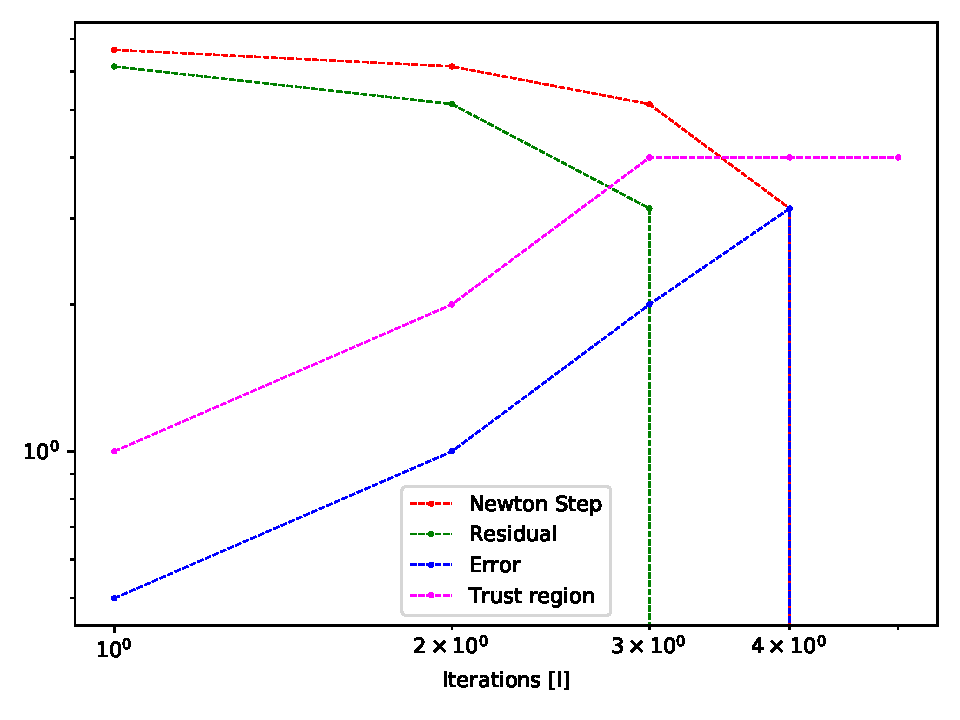
\includegraphics[width=1\linewidth]{figures/trivial_500.pdf}
    \caption{500 equations}
    \label{fig:trivial_1}
    \end{subfigure}%
  \begin{subfigure}{.5\textwidth}
    \centering
    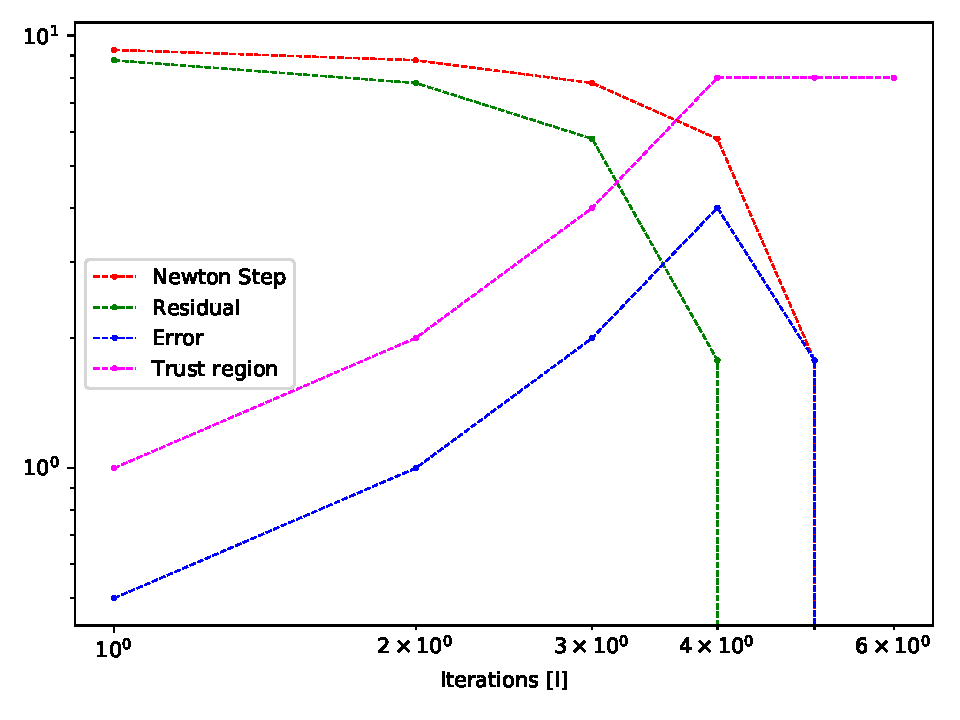
\includegraphics[width=1\linewidth]{figures/trivial_1000.pdf}
    \caption{1000 equations}
    \label{fig:trivial_2}
  \end{subfigure}
  \caption{Newton step size, residual, error, and trust region size vs. number of iterations for $\lambda = 0$.}
  \label{fig:trivial}
\end{figure}

The rate of convergence was tested for a range of number of equations with the same parameter values as for the trivial case. and the results are shown  in fig.~\ref{fig:conv}. As the number of equations increases, the 2 norm of the residuals increases (since it's proportional of $\sqrt{N}$), which explains the plateau as the number of equations increases. The plateau denotes the iterations which a used for arriving at a close enough approximation and beyong that the convergence is quadratic.
\begin{figure}
  \centering
  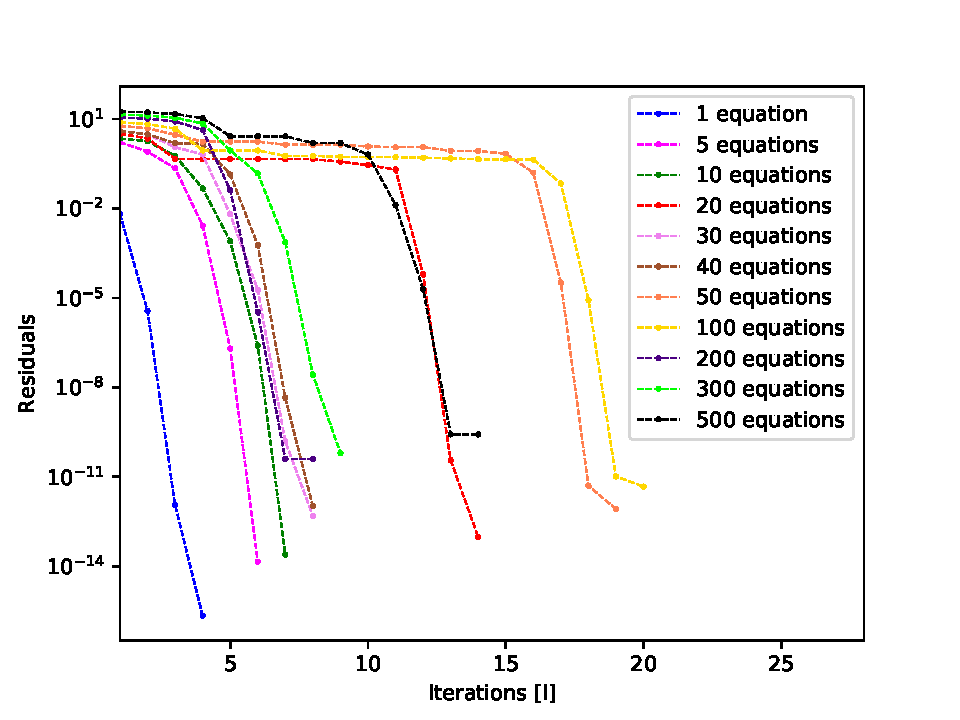
\includegraphics{figures/convergence.pdf}
  \caption{Convergence rate for the Newton-Hook method.}
  \label{}
\end{figure}



  \bibliography{references}
\end{document}
